\documentclass[12pt,a4paper]{article}
\usepackage[margin=1in]{geometry}
\usepackage{amsmath,amssymb,amsfonts}
\usepackage{graphicx}
\usepackage{hyperref}
\usepackage{listings}
\usepackage{xcolor}
\usepackage{booktabs}
\usepackage{longtable}
\usepackage{array}
\usepackage{multirow}
\usepackage{tikz}
\usetikzlibrary{shapes,arrows,positioning,fit,calc}
\usepackage{float}
\usepackage{enumitem}
\usepackage{fancyhdr}
\usepackage{titlesec}
\usepackage{tcolorbox}

\pagestyle{fancy}
\fancyhf{}
\rhead{CA Lab 3 -- Theory Document (Part 1)}
\lhead{ToyRISC Single-Cycle Processor}
\cfoot{\thepage}

\definecolor{codegreen}{rgb}{0,0.6,0}
\definecolor{codegray}{rgb}{0.5,0.5,0.5}
\definecolor{codepurple}{rgb}{0.58,0,0.82}
\definecolor{backcolour}{rgb}{0.95,0.95,0.92}

\lstdefinestyle{javastyle}{
    backgroundcolor=\color{backcolour},
    commentstyle=\color{codegreen},
    keywordstyle=\color{blue}\bfseries,
    numberstyle=\tiny\color{codegray},
    stringstyle=\color{codepurple},
    basicstyle=\ttfamily\footnotesize,
    breakatwhitespace=false,
    breaklines=true,
    captionpos=b,
    keepspaces=true,
    numbers=left,
    numbersep=5pt,
    showspaces=false,
    showstringspaces=false,
    showtabs=false,
    tabsize=2,
    frame=single
}

\lstdefinestyle{asmstyle}{
    backgroundcolor=\color{backcolour},
    commentstyle=\color{codegreen},
    keywordstyle=\color{blue}\bfseries,
    basicstyle=\ttfamily\footnotesize,
    breaklines=true,
    captionpos=b,
    keepspaces=true,
    numbers=left,
    numbersep=5pt,
    frame=single,
    morekeywords={add,addi,sub,subi,mul,muli,div,divi,and,andi,or,ori,xor,xori,slt,slti,sll,slli,srl,srli,sra,srai,load,store,jmp,beq,bne,blt,bgt,end}
}

\title{\Huge\bfseries Comprehensive Theory of Single-Cycle Processor Design and the ToyRISC ISA\\[1em]
\Large Part 1: Foundations of Computer Architecture}
\author{Computer Architecture Laboratory -- Assignment 3}
\date{\today}

\begin{document}

\maketitle
\tableofcontents
\newpage

% ===========================================================================
\section{Introduction to Computer Architecture}
% ===========================================================================

Computer architecture is the science and art of designing the fundamental operational structure of a computer system. It encompasses the instruction set architecture (ISA), the microarchitecture, and the system design. Understanding computer architecture is essential for writing efficient software, designing hardware, and bridging the gap between high-level programming and the actual hardware that executes programs.

\subsection{The Role of Computer Architecture}

At its core, a computer is a machine that fetches instructions from memory, decodes them, executes them, and stores results. Computer architecture defines:

\begin{itemize}[leftmargin=*]
    \item \textbf{What operations the processor can perform} -- defined by the Instruction Set Architecture (ISA).
    \item \textbf{How those operations are implemented in hardware} -- defined by the microarchitecture.
    \item \textbf{How the processor interacts with memory and I/O} -- defined by the system architecture.
\end{itemize}

\subsection{Levels of Abstraction}

Computer systems are organized in layers of abstraction, from high-level software to the transistors of the chip:

\begin{enumerate}
    \item \textbf{Application Software}: Programs written in high-level languages (C, Java, Python).
    \item \textbf{System Software}: Operating systems, compilers, assemblers that translate and manage.
    \item \textbf{Instruction Set Architecture (ISA)}: The contract between hardware and software. Defines registers, instructions, memory model, and data types.
    \item \textbf{Microarchitecture}: The implementation of the ISA in hardware. Includes pipeline design, cache hierarchy, branch prediction, etc.
    \item \textbf{Register-Transfer Level (RTL)}: The description of data flow between registers and the combinational logic that transforms data.
    \item \textbf{Gate Level}: Logic gates (AND, OR, NOT, XOR, MUX) that implement the RTL.
    \item \textbf{Transistor Level}: Physical CMOS transistors that implement the gates.
\end{enumerate}

\subsection{Von Neumann Architecture}

The Von Neumann architecture, proposed by John von Neumann in 1945, is the foundation of nearly all modern computers. Its key principles are:

\begin{enumerate}
    \item \textbf{Stored Program Concept}: Both instructions and data reside in the same memory. This allows programs to be modified, loaded dynamically, and treated as data.
    \item \textbf{Sequential Execution}: Instructions are fetched and executed one at a time, in the order they appear in memory (unless a branch or jump alters control flow).
    \item \textbf{Single Memory Space}: A unified address space holds both code and data (though the ToyRISC ISA separates them logically into segments).
    \item \textbf{Central Processing Unit (CPU)}: Contains the Arithmetic Logic Unit (ALU) for computation and the Control Unit (CU) for sequencing operations.
\end{enumerate}

The \textbf{Von Neumann bottleneck} is the limitation that arises because the CPU can only fetch one instruction or one data value per memory access cycle. This bottleneck motivates caches, pipelining, and Harvard architecture variants.

\subsection{Harvard Architecture}

The Harvard architecture separates instruction memory from data memory, allowing simultaneous access to both. Many modern processors use a \textbf{modified Harvard architecture}, which has separate instruction and data caches (L1i and L1d) but a unified main memory. The ToyRISC simulator's configuration file includes parameters for both L1i and L1d caches, reflecting this design philosophy.

% ===========================================================================
\section{Instruction Set Architecture (ISA) -- General Theory}
% ===========================================================================

The ISA is the most important abstraction in computer architecture. It defines the interface between software and hardware.

\subsection{What an ISA Defines}

An ISA specifies the following:

\begin{itemize}[leftmargin=*]
    \item \textbf{Data Types}: Integer (signed/unsigned), floating point, character, boolean. ToyRISC uses 32-bit signed integers.
    \item \textbf{Registers}: The number, size, and purpose of registers. ToyRISC has 32 general-purpose registers (\texttt{x0}--\texttt{x31}), each 32 bits wide.
    \item \textbf{Instruction Formats}: The binary encoding of instructions. ToyRISC uses 32-bit fixed-width instructions in three formats (R3-Type, R2I-Type, RI-Type).
    \item \textbf{Instruction Types}: Arithmetic, logical, memory access, control flow, and special instructions.
    \item \textbf{Addressing Modes}: How operand addresses are computed. ToyRISC supports register, immediate, and register+immediate (base+offset) addressing.
    \item \textbf{Memory Model}: Address space size, byte ordering, alignment. ToyRISC has a 16-bit address space ($2^{16} = 65536$ words).
    \item \textbf{Exception and Interrupt Handling}: How the processor responds to errors and external events (not covered in ToyRISC).
\end{itemize}

\subsection{RISC vs. CISC}

\subsubsection{CISC (Complex Instruction Set Computer)}

CISC architectures (e.g., x86) have:
\begin{itemize}
    \item Variable-length instructions (1 to 15 bytes in x86).
    \item Complex instructions that can perform multiple operations (e.g., REP MOVSB moves a block of memory).
    \item Many addressing modes (register, immediate, direct, indirect, indexed, based+indexed, etc.).
    \item Fewer registers (historically 8 in x86).
    \item Microprogrammed control units.
\end{itemize}

\subsubsection{RISC (Reduced Instruction Set Computer)}

RISC architectures (e.g., MIPS, ARM, RISC-V, and ToyRISC) have:
\begin{itemize}
    \item Fixed-length instructions (32 bits in ToyRISC).
    \item Simple instructions that each perform one operation.
    \item Load-store architecture: only \texttt{load} and \texttt{store} access memory; all other operations work on registers.
    \item Many general-purpose registers (32 in ToyRISC, same as RISC-V and MIPS).
    \item Hardwired control units.
    \item Regular instruction formats that simplify decoding.
\end{itemize}

ToyRISC is a classic RISC architecture. It follows the load-store paradigm, has fixed 32-bit instructions, and uses a simple, regular encoding scheme.

\subsection{Instruction Encoding Fundamentals}

Every instruction must be encoded as a binary number. The encoding must contain enough information for the processor to determine:

\begin{enumerate}
    \item \textbf{What operation to perform} (opcode).
    \item \textbf{What data to operate on} (operands: register numbers, immediate values).
    \item \textbf{Where to put the result} (destination register or memory address).
\end{enumerate}

In a fixed-width ISA like ToyRISC (32 bits per instruction), the challenge is to pack all this information into a fixed number of bits. This requires trade-offs:
\begin{itemize}
    \item More bits for the opcode $\Rightarrow$ more distinct operations but fewer bits for operands.
    \item More bits for immediate values $\Rightarrow$ larger constants but fewer bits for register specifiers.
    \item More register specifier fields $\Rightarrow$ more operands but smaller immediates.
\end{itemize}

\subsection{Addressing Modes}

Addressing modes define how the processor computes the effective address of an operand:

\begin{longtable}{p{4cm}p{4cm}p{5cm}}
\toprule
\textbf{Mode} & \textbf{Example} & \textbf{Description} \\
\midrule
Register & \texttt{add x3, x4, x5} & Operand is in a register \\
Immediate & \texttt{addi x3, 5, x5} & Operand is a constant embedded in the instruction \\
Base + Offset & \texttt{load x3, 10, x5} & Memory address = register value + immediate \\
PC-Relative & \texttt{beq x3, x4, label} & Branch target = PC + offset \\
\bottomrule
\end{longtable}

ToyRISC uses all four of these modes. The base+offset mode is used by \texttt{load} and \texttt{store}. PC-relative mode is used by conditional branches (\texttt{beq}, \texttt{bne}, \texttt{blt}, \texttt{bgt}) and unconditional jumps (\texttt{jmp}).

% ===========================================================================
\section{Registers and the Register File}
% ===========================================================================

\subsection{What are Registers?}

Registers are the fastest storage elements in a processor. They are implemented using flip-flops (latches) within the CPU itself, so accessing a register takes zero additional clock cycles beyond the pipeline stage that reads them. By contrast, main memory access can take tens to hundreds of clock cycles.

\subsection{The ToyRISC Register File}

ToyRISC has \textbf{32 general-purpose integer registers}, each 32 bits wide, denoted \texttt{x0} through \texttt{x31}. Additionally, there is a \textbf{Program Counter (PC)} register that holds the address of the current instruction.

\subsubsection{Special Registers}

\begin{longtable}{p{2cm}p{3cm}p{8cm}}
\toprule
\textbf{Register} & \textbf{Name} & \textbf{Purpose} \\
\midrule
\texttt{x0} & Zero Register & Always contains the value 0. Cannot be overwritten. Used as a source of zero for operations like clearing a register (\texttt{add x0, x0, x3} sets \texttt{x3 = 0}). \\
\texttt{x1} & Stack Pointer (SP) & Points to the top of the stack. Initialized to $2^{16} - 1 = 65535$. The stack grows downward (toward lower addresses). \\
\texttt{x2} & Frame Pointer (FP) & Points to the base of the current stack frame. Initialized to $2^{16} - 1 = 65535$. Used to access function arguments and local variables at fixed offsets. \\
\texttt{x31} & Overflow / Remainder & Stores the upper 32 bits of a 64-bit multiplication result, the remainder of a division, or the bits shifted out during shift operations. \\
PC & Program Counter & Holds the memory address of the instruction currently being fetched. Incremented by 1 after each fetch (since each instruction occupies one memory word). \\
\bottomrule
\end{longtable}

\subsection{Register File Implementation}

In the Java simulator, the register file is implemented by the \texttt{RegisterFile.java} class:

\begin{lstlisting}[style=javastyle, caption={RegisterFile.java -- Simplified}]
public class RegisterFile {
    int[] registerFile;  // 32 registers, each 32-bit int
    int programCounter;  // PC register

    public RegisterFile() {
        registerFile = new int[32];
        registerFile[0] = 0;  // x0 is always 0
    }

    public int getValue(int registerNumber) {
        return registerFile[registerNumber];
    }

    public void setValue(int registerNumber, int value) {
        registerFile[registerNumber] = value;
    }

    public int getProgramCounter() {
        return programCounter;
    }

    public void setProgramCounter(int programCounter) {
        this.programCounter = programCounter;
    }

    public void incrementProgramCounter() {
        this.programCounter++;
    }
}
\end{lstlisting}

Key observations:
\begin{itemize}
    \item The register file is a simple array of 32 integers.
    \item The PC is stored as a separate integer field.
    \item Register numbering requires 5 bits ($\log_2 32 = 5$), which is why each register specifier in the instruction format is 5 bits.
    \item In a real hardware implementation, the register file would have multiple read ports (typically 2) and one write port, allowing the processor to read two source registers and write one destination register simultaneously.
\end{itemize}

% ===========================================================================
\section{Memory System}
% ===========================================================================

\subsection{Main Memory in ToyRISC}

The ToyRISC processor has a \textbf{word-addressable} main memory with $2^{16} = 65536$ words. Each word is 32 bits (an \texttt{int} in Java). This means the total memory capacity is:
\[
65536 \times 32 \text{ bits} = 65536 \times 4 \text{ bytes} = 262144 \text{ bytes} = 256 \text{ KB}
\]

Note that ToyRISC uses \textbf{word addressing}, not byte addressing. Address 0 refers to the first 32-bit word, address 1 refers to the second 32-bit word, and so on. This is different from most real architectures (x86, ARM, RISC-V) which use byte addressing.

\subsection{Address Space Layout}

The ToyRISC address space is divided into three segments:

\begin{figure}[H]
\centering
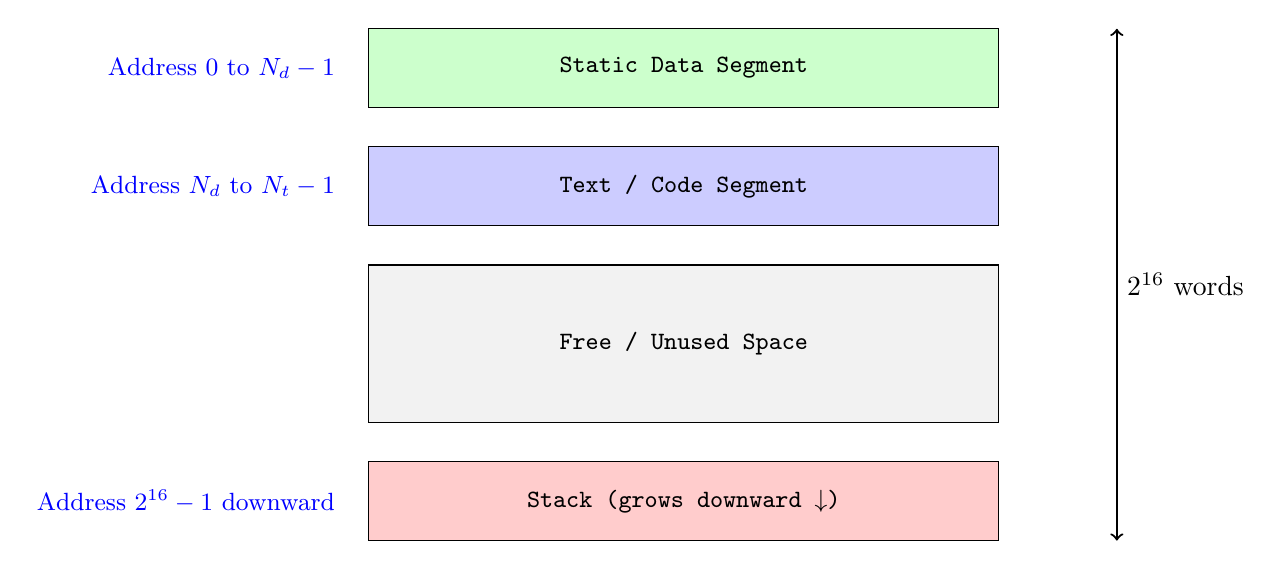
\begin{tikzpicture}[
    block/.style={draw, rectangle, minimum width=8cm, minimum height=1cm, text centered, font=\ttfamily\small},
    label/.style={font=\small, text=blue}
]
\node[block, fill=green!20] (data) at (0,5) {Static Data Segment};
\node[label, left=0.3cm of data] {Address 0 to $N_d - 1$};

\node[block, fill=blue!20] (text) at (0,3.5) {Text / Code Segment};
\node[label, left=0.3cm of text] {Address $N_d$ to $N_t - 1$};

\node[block, fill=gray!10, minimum height=2cm] (free) at (0,1.5) {Free / Unused Space};

\node[block, fill=red!20] (stack) at (0,-0.5) {Stack (grows downward $\downarrow$)};
\node[label, left=0.3cm of stack] {Address $2^{16} - 1$ downward};

\draw[<->, thick] (5.5,5.5) -- (5.5,-1) node[midway, right] {$2^{16}$ words};
\end{tikzpicture}
\caption{ToyRISC Address Space Layout}
\end{figure}

\subsubsection{Static Data Segment (Address 0 to $N_d - 1$)}

The static data segment starts at address 0 and contains global variables and constants declared in the \texttt{.data} section of the assembly program. For example:

\begin{lstlisting}[style=asmstyle]
.data
a:
    123
    234
\end{lstlisting}

Here, value 123 is stored at address 0, and value 234 is stored at address 1. The label \texttt{a} is an alias for address 0.

\subsubsection{Text / Code Segment (Address $N_d$ to $N_t - 1$)}

The text segment immediately follows the data segment. It contains the machine code instructions of the program. Each instruction occupies exactly one 32-bit word (one memory address). If the data segment contains $N_d$ words, then the first instruction is at address $N_d$.

\subsubsection{Stack Segment (Address $2^{16} - 1$ downward)}

The stack starts at the highest address ($2^{16} - 1 = 65535$) and grows \textbf{downward} (toward lower addresses). The stack pointer (\texttt{x1}) and frame pointer (\texttt{x2}) are both initialized to 65535.

\textbf{Push operation}: Decrement the stack pointer by 1, then store the value at the address pointed to by the stack pointer.

\textbf{Pop operation}: Load the value from the address pointed to by the stack pointer, then increment the stack pointer by 1.

\subsection{Memory Implementation}

\begin{lstlisting}[style=javastyle, caption={MainMemory.java}]
public class MainMemory {
    int[] memory;

    public MainMemory() {
        memory = new int[65536];  // 2^16 words
    }

    public int getWord(int address) {
        return memory[address];
    }

    public void setWord(int address, int value) {
        memory[address] = value;
    }
}
\end{lstlisting}

\subsection{Memory Hierarchy (Preview)}

While the single-cycle simulator in Lab 3 does not implement caches, the configuration file (\texttt{config.xml}) defines a memory hierarchy for future assignments:

\begin{enumerate}
    \item \textbf{L1 Instruction Cache (L1i)}: 256 lines, 2-cycle latency, 4-way set-associative, LRU replacement.
    \item \textbf{L1 Data Cache (L1d)}: 256 lines, 2-cycle latency, 4-way set-associative, LRU replacement.
    \item \textbf{L2 Unified Cache}: 2048 lines, 10-cycle latency, 4-way set-associative, LRU replacement.
    \item \textbf{Main Memory}: 40-cycle latency.
\end{enumerate}

This hierarchy illustrates the principle of \textbf{locality of reference}: recently accessed data (temporal locality) and nearby data (spatial locality) are likely to be accessed again soon, so keeping them in fast, small caches dramatically improves performance.

% ===========================================================================
\section{The Single-Cycle Processor Model}
% ===========================================================================

\subsection{What is a Single-Cycle Processor?}

A single-cycle processor executes \textbf{one instruction per clock cycle} (or equivalently, one instruction passes through all stages before the next begins). In this model:

\begin{itemize}
    \item The clock period must be long enough to accommodate the \textbf{slowest instruction} (typically a load instruction, which requires memory access).
    \item All instructions take the same amount of time, even simple ones like \texttt{add} that don't need memory access.
    \item There is no overlap between instructions -- no pipelining.
\end{itemize}

\subsection{Stages of Instruction Execution}

Every instruction, regardless of type, passes through the same sequence of stages:

\begin{figure}[H]
\centering
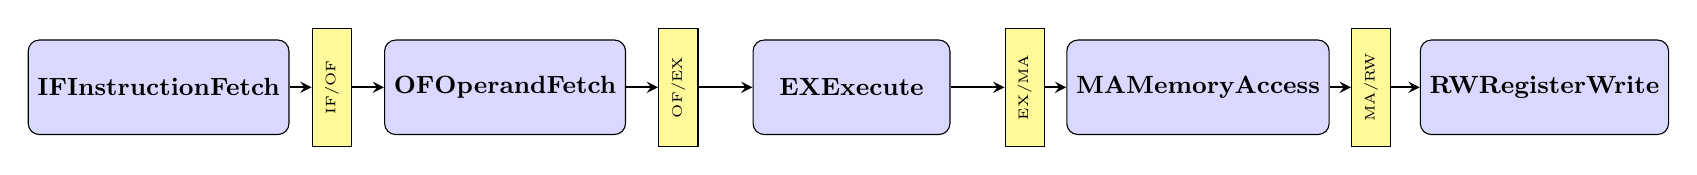
\begin{tikzpicture}[
    stage/.style={draw, rectangle, rounded corners, minimum width=2.5cm, minimum height=1.2cm, text centered, font=\bfseries\small, fill=blue!15},
    latch/.style={draw, rectangle, minimum width=0.5cm, minimum height=1.5cm, fill=yellow!40, font=\tiny},
    arrow/.style={->, thick, >=stealth}
]
\node[stage] (IF) at (0,0) {IF\\Instruction\\Fetch};
\node[latch] (l1) at (2.2,0) {\rotatebox{90}{IF/OF}};
\node[stage] (OF) at (4.4,0) {OF\\Operand\\Fetch};
\node[latch] (l2) at (6.6,0) {\rotatebox{90}{OF/EX}};
\node[stage] (EX) at (8.8,0) {EX\\Execute};
\node[latch] (l3) at (11,0) {\rotatebox{90}{EX/MA}};
\node[stage] (MA) at (13.2,0) {MA\\Memory\\Access};
\node[latch] (l4) at (15.4,0) {\rotatebox{90}{MA/RW}};
\node[stage] (RW) at (17.6,0) {RW\\Register\\Write};

\draw[arrow] (IF) -- (l1);
\draw[arrow] (l1) -- (OF);
\draw[arrow] (OF) -- (l2);
\draw[arrow] (l2) -- (EX);
\draw[arrow] (EX) -- (l3);
\draw[arrow] (l3) -- (MA);
\draw[arrow] (MA) -- (l4);
\draw[arrow] (l4) -- (RW);
\end{tikzpicture}
\caption{Five-Stage Single-Cycle Pipeline with Inter-Stage Latches}
\end{figure}

\subsubsection{Stage 1: Instruction Fetch (IF)}

\textbf{Purpose}: Retrieve the next instruction from memory.

\textbf{Actions}:
\begin{enumerate}
    \item Read the Program Counter (PC) to get the address of the current instruction.
    \item Access main memory at that address to fetch the 32-bit instruction word.
    \item Increment the PC by 1 (pointing to the next sequential instruction).
    \item Write the fetched instruction into the IF/OF latch.
\end{enumerate}

\textbf{Hardware components used}: Program Counter register, instruction memory (or instruction cache), adder (for PC+1).

\textbf{Java implementation} (provided in the skeleton):
\begin{lstlisting}[style=javastyle, caption={InstructionFetch.java -- performIF()}]
public void performIF() {
    if(IF_EnableLatch.isIF_enable()) {
        int currentPC = containingProcessor.getRegisterFile()
                        .getProgramCounter();
        int newInstruction = containingProcessor.getMainMemory()
                             .getWord(currentPC);
        IF_OF_Latch.setInstruction(newInstruction);
        containingProcessor.getRegisterFile()
                          .setProgramCounter(currentPC + 1);

        IF_EnableLatch.setIF_enable(false);
        IF_OF_Latch.setOF_enable(true);
    }
}
\end{lstlisting}

\subsubsection{Stage 2: Operand Fetch / Instruction Decode (OF/ID)}

\textbf{Purpose}: Decode the instruction and read the required register values.

\textbf{Actions}:
\begin{enumerate}
    \item Read the 32-bit instruction word from the IF/OF latch.
    \item Extract the opcode (bits 27--31) to determine the operation type.
    \item Based on the instruction format (R3-Type, R2I-Type, or RI-Type), extract:
    \begin{itemize}
        \item Source register 1 (\texttt{rs1}) -- bits 22--26
        \item Source register 2 (\texttt{rs2}) or immediate -- depends on format
        \item Destination register (\texttt{rd}) -- depends on format
    \end{itemize}
    \item Read the values of the source registers from the register file.
    \item Sign-extend the immediate value (if applicable).
    \item Write all decoded information into the OF/EX latch.
\end{enumerate}

\textbf{Hardware components used}: Instruction decoder (combinational logic), register file (read ports), sign extender, multiplexers.

\subsubsection{Stage 3: Execute (EX)}

\textbf{Purpose}: Perform the computation specified by the instruction.

\textbf{Actions} (depend on instruction type):
\begin{itemize}
    \item \textbf{Arithmetic/Logical}: Compute the result using the ALU (e.g., add, subtract, multiply, divide, AND, OR, XOR, SLT, shifts).
    \item \textbf{Memory}: Compute the effective address: base register + immediate offset.
    \item \textbf{Branch}: Compare the two source registers and determine whether the branch is taken. If taken, compute the target address: PC + immediate offset.
    \item \textbf{Jump}: Compute the target address: PC + rd + immediate.
\end{itemize}

\textbf{Hardware components used}: Arithmetic Logic Unit (ALU), comparator, adder, barrel shifter, multiplier, divider.

\subsubsection{Stage 4: Memory Access (MA)}

\textbf{Purpose}: Access data memory for load and store instructions.

\textbf{Actions}:
\begin{itemize}
    \item \textbf{Load}: Read the data word from main memory at the effective address computed in the EX stage.
    \item \textbf{Store}: Write the data word to main memory at the effective address.
    \item \textbf{Other instructions}: This stage is a pass-through (no memory operation needed).
\end{itemize}

\textbf{Hardware components used}: Data memory (or data cache), address bus, data bus.

\subsubsection{Stage 5: Register Write-Back (RW)}

\textbf{Purpose}: Write the result of the instruction back to the register file.

\textbf{Actions}:
\begin{itemize}
    \item \textbf{Arithmetic/Logical}: Write the ALU result to the destination register.
    \item \textbf{Load}: Write the loaded data to the destination register.
    \item \textbf{Store}: No register write needed.
    \item \textbf{Branch/Jump}: No register write needed (but PC may have been updated in EX stage).
    \item \textbf{End}: Signal simulation completion.
\end{itemize}

\textbf{Hardware components used}: Register file (write port), multiplexer to select between ALU result and memory data.

\subsection{The Clock and Timing}

In a single-cycle processor:
\[
T_{\text{clock}} \geq T_{\text{IF}} + T_{\text{OF}} + T_{\text{EX}} + T_{\text{MA}} + T_{\text{RW}}
\]

The clock period must be long enough for the signal to propagate through \textbf{all five stages} in a single cycle. This is determined by the critical path, which is typically the \texttt{load} instruction (it uses all five stages actively).

For ToyRISC in the simulator, the clock is simply a counter:

\begin{lstlisting}[style=javastyle, caption={Clock.java}]
public class Clock {
    static long currentTime = 0;

    public static void incrementClock() {
        currentTime++;
    }

    public static long getCurrentTime() {
        return currentTime;
    }
}
\end{lstlisting}

In the \texttt{simulate()} function, the clock increments after each stage:

\begin{lstlisting}[style=javastyle, caption={Simulator.java -- simulate() loop}]
public static void simulate() {
    while(simulationComplete == false) {
        processor.getIFUnit().performIF();
        Clock.incrementClock();
        processor.getOFUnit().performOF();
        Clock.incrementClock();
        processor.getEXUnit().performEX();
        Clock.incrementClock();
        processor.getMAUnit().performMA();
        Clock.incrementClock();
        processor.getRWUnit().performRW();
        Clock.incrementClock();
    }
}
\end{lstlisting}

Each instruction takes \textbf{5 clock ticks} (one per stage). This is the single-cycle model: one complete instruction per 5-tick ``cycle.''

\subsection{Performance Metrics}

For a single-cycle processor:

\begin{itemize}
    \item \textbf{CPI (Cycles Per Instruction)} = 1 instruction per ``instruction cycle'' (but each instruction cycle is 5 clock ticks in the simulator).
    \item \textbf{Execution Time} = Number of Instructions $\times$ CPI $\times$ Clock Period
    \item \textbf{Throughput} = $\frac{1}{\text{Clock Period}}$ instructions per second
    \item \textbf{Latency} = Time to complete one instruction = Clock Period
\end{itemize}

The number of cycles reported by the simulator is $5 \times$ (number of instructions), since the clock increments 5 times per instruction.

\subsection{Advantages and Disadvantages}

\begin{tcolorbox}[colback=green!5, colframe=green!50!black, title=Advantages of Single-Cycle Design]
\begin{itemize}
    \item \textbf{Simplicity}: No hazard detection, no forwarding, no stalling.
    \item \textbf{Correctness}: Easy to verify because there's no overlap between instructions.
    \item \textbf{Deterministic}: Every instruction takes exactly the same time.
    \item \textbf{No pipeline hazards}: Data hazards, control hazards, and structural hazards don't exist.
\end{itemize}
\end{tcolorbox}

\begin{tcolorbox}[colback=red!5, colframe=red!50!black, title=Disadvantages of Single-Cycle Design]
\begin{itemize}
    \item \textbf{Slow}: The clock period is determined by the slowest instruction. Simple instructions (like \texttt{add}) are unnecessarily slow.
    \item \textbf{Poor resource utilization}: Most hardware components are idle for most of the clock cycle. The ALU is only active during the EX stage; memory is only active during IF and MA.
    \item \textbf{Not scalable}: As the ISA grows more complex, the critical path lengthens, and the clock period must increase.
\end{itemize}
\end{tcolorbox}

% ===========================================================================
\section{Inter-Stage Latches}
% ===========================================================================

\subsection{Purpose of Latches}

In a processor pipeline (even a single-cycle one simulated sequentially), \textbf{latches} (also called \textbf{pipeline registers}) are buffers that sit between two consecutive stages. They serve two purposes:

\begin{enumerate}
    \item \textbf{Communication}: They pass the output of one stage to the input of the next stage.
    \item \textbf{Synchronization}: In a pipelined processor, they ensure that each stage works on a different instruction simultaneously. In a single-cycle processor, they simply hold intermediate results.
\end{enumerate}

\subsection{ToyRISC Latch Types}

The ToyRISC simulator has the following latches:

\begin{longtable}{p{4cm}p{3cm}p{6cm}}
\toprule
\textbf{Latch} & \textbf{Between Stages} & \textbf{Contents} \\
\midrule
\texttt{IF\_EnableLatchType} & Enable $\to$ IF & Boolean: whether IF stage should execute \\
\texttt{IF\_OF\_LatchType} & IF $\to$ OF & The 32-bit instruction word; OF enable flag \\
\texttt{OF\_EX\_LatchType} & OF $\to$ EX & Decoded instruction (opcode, source operand values, destination register, immediate), EX enable flag \\
\texttt{EX\_MA\_LatchType} & EX $\to$ MA & ALU result, effective address, data to store, MA enable flag \\
\texttt{EX\_IF\_LatchType} & EX $\to$ IF & Branch/jump target PC (for control flow instructions) \\
\texttt{MA\_RW\_LatchType} & MA $\to$ RW & ALU result or loaded data, destination register, RW enable flag \\
\bottomrule
\end{longtable}

Note the \texttt{EX\_IF\_LatchType}: this is a \textbf{feedback latch} from the Execute stage back to the Instruction Fetch stage. It is used when a branch or jump instruction needs to redirect the PC.

\subsection{Latch as a Handshake Mechanism}

Each latch has an ``enable'' flag that implements a simple handshake:
\begin{enumerate}
    \item Stage $N$ completes its work and writes results to the $N$/$N{+}1$ latch.
    \item Stage $N$ sets the enable flag of Stage $N{+}1$ to \texttt{true}.
    \item Stage $N{+}1$ checks its enable flag; if \texttt{true}, it proceeds.
    \item Stage $N{+}1$ sets its own enable flag to \texttt{false} after reading.
\end{enumerate}

For example, in \texttt{InstructionFetch.performIF()}:
\begin{lstlisting}[style=javastyle]
IF_EnableLatch.setIF_enable(false);  // disable IF
IF_OF_Latch.setOF_enable(true);     // enable OF
\end{lstlisting}

% ===========================================================================
\section{The Instruction Lifecycle -- Complete Walkthrough}
% ===========================================================================

Let us trace the complete lifecycle of an instruction through all five stages using a concrete example:

\textbf{Example}: \texttt{add \%x3, \%x4, \%x5} (add values in registers x3 and x4, store result in x5)

Assume: \texttt{x3 = 10}, \texttt{x4 = 20}, PC = 5 (instruction at memory address 5).

\subsection{Step 1: Instruction Fetch (IF)}

\begin{enumerate}
    \item Read PC = 5.
    \item Fetch instruction from \texttt{memory[5]}. This returns the 32-bit binary encoding of \texttt{add \%x3, \%x4, \%x5}.
    \item Increment PC to 6.
    \item Write the 32-bit instruction to the IF/OF latch.
    \item Set OF enable = true, IF enable = false.
\end{enumerate}

\subsection{Step 2: Operand Fetch (OF)}

\begin{enumerate}
    \item Read the 32-bit instruction from the IF/OF latch.
    \item Extract opcode = 00000 (add).
    \item This is R3-Type, so extract: rs1 = x3 (bits 22--26), rs2 = x4 (bits 17--21), rd = x5 (bits 12--16).
    \item Read register file: \texttt{x3} = 10, \texttt{x4} = 20.
    \item Write to OF/EX latch: opcode = add, operand1 = 10, operand2 = 20, destination = x5.
    \item Set EX enable = true, OF enable = false.
\end{enumerate}

\subsection{Step 3: Execute (EX)}

\begin{enumerate}
    \item Read from OF/EX latch: opcode = add, operand1 = 10, operand2 = 20.
    \item Compute: result = 10 + 20 = 30.
    \item Write to EX/MA latch: result = 30, destination = x5.
    \item Set MA enable = true, EX enable = false.
\end{enumerate}

\subsection{Step 4: Memory Access (MA)}

\begin{enumerate}
    \item Read from EX/MA latch: result = 30, instruction type = add.
    \item Since \texttt{add} is not a memory instruction, this is a pass-through.
    \item Write to MA/RW latch: result = 30, destination = x5.
    \item Set RW enable = true, MA enable = false.
\end{enumerate}

\subsection{Step 5: Register Write (RW)}

\begin{enumerate}
    \item Read from MA/RW latch: result = 30, destination = x5.
    \item Write 30 to register x5.
    \item Set IF enable = true (allowing the next instruction to be fetched).
    \item Set RW enable = false.
\end{enumerate}

\textbf{Result}: Register x5 now contains 30. PC = 6 (ready to fetch next instruction).

% ===========================================================================
\section{Number Representation and Binary Arithmetic}
% ===========================================================================

\subsection{Two's Complement Representation}

ToyRISC uses 32-bit signed integers in two's complement. In two's complement:

\begin{itemize}
    \item The most significant bit (bit 31) is the \textbf{sign bit}: 0 for positive, 1 for negative.
    \item Range: $-2^{31}$ to $2^{31} - 1$ (i.e., $-2,147,483,648$ to $2,147,483,647$).
    \item To negate a number: invert all bits and add 1.
    \item Addition and subtraction use the same hardware circuit, which is why two's complement is universal in computer architecture.
\end{itemize}

\subsection{Sign Extension}

When an immediate value with fewer bits (e.g., 17 bits in R2I-Type or 22 bits in RI-Type) needs to be used in a 32-bit operation, it must be \textbf{sign-extended}: the sign bit is replicated to fill the upper bits.

For example, a 17-bit immediate value of $-5$:
\begin{itemize}
    \item 17-bit: \texttt{1 1111 1111 1111 1011}
    \item 32-bit (sign-extended): \texttt{1111 1111 1111 1111 1111 1111 1111 1011}
\end{itemize}

\subsection{Overflow and Special Handling in ToyRISC}

According to the ISA specification:
\begin{itemize}
    \item \textbf{Multiplication}: If the 64-bit result exceeds 32 bits, the upper 32 bits (bits 63--32) are stored in \texttt{x31}.
    \item \textbf{Division}: The quotient goes to the destination register, and the \textbf{remainder} goes to \texttt{x31}.
    \item \textbf{Shifts}: The bits shifted out are stored in \texttt{x31}.
\end{itemize}

\subsection{Bitwise Operations}

ToyRISC supports the standard bitwise operations:

\begin{longtable}{p{2cm}p{3cm}p{8cm}}
\toprule
\textbf{Operation} & \textbf{Symbol} & \textbf{Description} \\
\midrule
AND & \texttt{\&} & Bitwise AND. Result bit is 1 only if both input bits are 1. \\
OR & \texttt{|} & Bitwise OR. Result bit is 1 if either input bit is 1. \\
XOR & \texttt{\^{}} & Bitwise XOR. Result bit is 1 if inputs differ. \\
SLL & $\ll$ & Shift Left Logical. Shifts bits left, fills right with zeros. \\
SRL & $\gg$ (logical) & Shift Right Logical. Shifts bits right, fills left with zeros. \\
SRA & $\gg$ (arith.) & Shift Right Arithmetic. Shifts bits right, fills left with sign bit (preserves sign). \\
\bottomrule
\end{longtable}

\newpage
% ===========================================================================
\section{Control Flow and Branching}
% ===========================================================================

\subsection{Sequential Execution}

By default, instructions execute sequentially: after executing the instruction at address $A$, the next instruction fetched is at address $A + 1$. This is achieved by incrementing the PC in the IF stage.

\subsection{Unconditional Jump (jmp)}

The \texttt{jmp} instruction changes the PC unconditionally:
\[
\text{PC} = \text{PC} + \text{rd} + \text{imm}
\]

In assembly, either \texttt{rd} or \texttt{imm} is used (the other is set to zero). For example:
\begin{lstlisting}[style=asmstyle]
jmp loop       ; Jump to the label 'loop'
\end{lstlisting}

In machine code, the label is converted to a PC-relative offset. If the current PC is 10 and the label \texttt{loop} is at address 7, then the offset would be $7 - 10 = -3$ (since $\text{PC}_{\text{new}} = \text{PC} + \text{offset}$). However, note that the PC has already been incremented by 1 during the IF stage, so the actual offset stored needs to account for this.

\subsection{Conditional Branches}

ToyRISC has four conditional branch instructions:

\begin{longtable}{p{2cm}p{3cm}p{8cm}}
\toprule
\textbf{Instruction} & \textbf{Condition} & \textbf{Action} \\
\midrule
\texttt{beq} & rs1 == rd & If true, PC = PC + imm \\
\texttt{bne} & rs1 $\neq$ rd & If true, PC = PC + imm \\
\texttt{blt} & rs1 < rd & If true, PC = PC + imm \\
\texttt{bgt} & rs1 > rd & If true, PC = PC + imm \\
\bottomrule
\end{longtable}

\textbf{Important}: In the \texttt{ParsedProgram} (object file) representation:
\begin{itemize}
    \item The two registers being compared are placed in \texttt{sourceOperand1} and \texttt{sourceOperand2}.
    \item The immediate offset is placed in \texttt{destinationOperand}.
\end{itemize}

This is a critical implementation detail for the Operand Fetch stage.

\subsection{Branch Target Calculation}

For branches, the target address is computed \textbf{relative to the current PC}:
\[
\text{Target} = \text{PC}_{\text{at branch}} + \text{imm}
\]

Since PC has already been incremented during IF, the actual target computed in EX is:
\[
\text{Target} = \text{PC}_{\text{original}} + \text{imm}
\]

The EX stage communicates the new PC back to the IF stage via the \texttt{EX\_IF\_LatchType}.

% ===========================================================================
\section{Function Calling Convention}
% ===========================================================================

The ToyRISC ISA defines a standard calling convention for function calls, specifying how arguments are passed, how the stack is managed, and how control is transferred.

\subsection{Stack Operations}

\textbf{Push} (storing a value onto the stack):
\begin{enumerate}
    \item Decrement x1 (stack pointer) by 1.
    \item Store the value at the address pointed to by x1.
\end{enumerate}

\textbf{Pop} (retrieving a value from the stack):
\begin{enumerate}
    \item Load the value from the address pointed to by x1.
    \item Increment x1 by 1.
\end{enumerate}

\subsection{Caller Responsibilities}

Before calling a function:
\begin{enumerate}
    \item \textbf{Save caller-saved registers}: Push any registers whose values the caller needs preserved.
    \item \textbf{Push arguments}: Push function arguments onto the stack.
    \item \textbf{Push return address}: Push the address of the instruction following the \texttt{jmp} to the function.
    \item \textbf{Jump to function}: Execute \texttt{jmp} to the function's entry point.
\end{enumerate}

After the function returns:
\begin{enumerate}
    \item Read return values from addresses below x1.
    \item Pop the previously saved registers.
\end{enumerate}

\subsection{Callee Responsibilities}

Upon entering the function:
\begin{enumerate}
    \item \textbf{Save x2}: Push the old frame pointer (x2) onto the stack.
    \item \textbf{Set up frame}: x2 = x1 - 1 (frame pointer points to the base of the current frame).
    \item \textbf{Perform computation}: Access arguments via x2 + offsets. Use stack space below x2 for local variables.
\end{enumerate}

Upon exiting the function:
\begin{enumerate}
    \item \textbf{Restore x1}: x1 = x2 (collapse the stack frame).
    \item \textbf{Restore x2}: Pop the saved frame pointer into x2.
    \item \textbf{Push return values}: Push return values onto the stack.
    \item \textbf{Return}: Load the return address from the stack and jump to it.
\end{enumerate}

\subsection{Stack Frame Layout}

\begin{figure}[H]
\centering
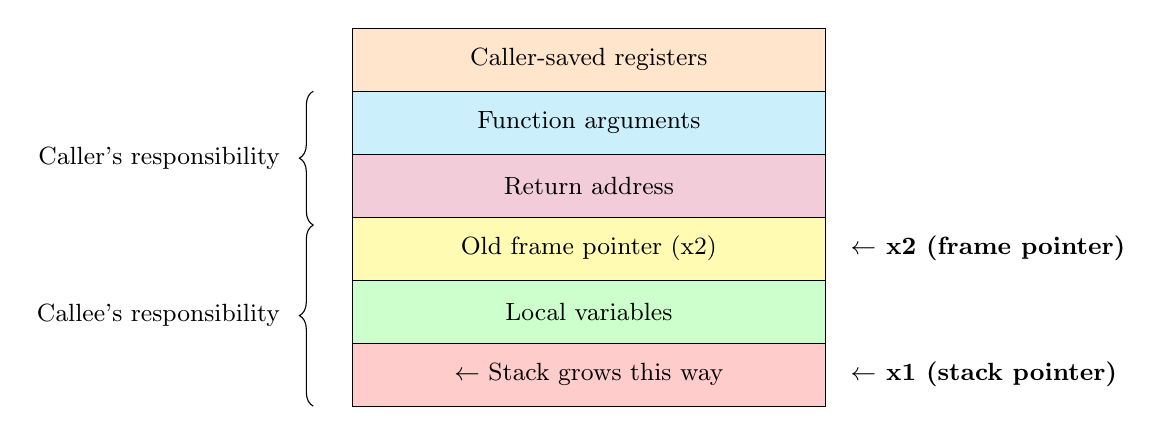
\begin{tikzpicture}[
    block/.style={draw, rectangle, minimum width=6cm, minimum height=0.8cm, text centered, font=\small},
]
\node[block, fill=orange!20] (callerregs) at (0,6) {Caller-saved registers};
\node[block, fill=cyan!20] (args) at (0,5.2) {Function arguments};
\node[block, fill=purple!20] (retaddr) at (0,4.4) {Return address};
\node[block, fill=yellow!30] (oldfp) at (0,3.6) {Old frame pointer (x2)};
\node[block, fill=green!20] (locals) at (0,2.8) {Local variables};
\node[block, fill=red!20] (grow) at (0,2.0) {$\leftarrow$ Stack grows this way};

\node[font=\small\bfseries, right=0.2cm] at (3,3.6) {$\leftarrow$ x2 (frame pointer)};
\node[font=\small\bfseries, right=0.2cm] at (3,2.0) {$\leftarrow$ x1 (stack pointer)};

\draw[decorate, decoration={brace, amplitude=5pt, mirror}] (-3.5,5.6) -- (-3.5,3.9) node[midway, left=0.3cm, font=\small] {Caller's responsibility};
\draw[decorate, decoration={brace, amplitude=5pt, mirror}] (-3.5,3.9) -- (-3.5,1.6) node[midway, left=0.3cm, font=\small] {Callee's responsibility};
\end{tikzpicture}
\caption{Stack Frame Layout in ToyRISC}
\end{figure}

% ===========================================================================
\section{Comparison with RISC-V}
% ===========================================================================

ToyRISC is intentionally designed to resemble RISC-V. Here is a comparison:

\begin{longtable}{p{4cm}p{5cm}p{5cm}}
\toprule
\textbf{Feature} & \textbf{ToyRISC} & \textbf{RISC-V (RV32I)} \\
\midrule
Word size & 32 bits & 32 bits \\
Registers & 32 (x0--x31) & 32 (x0--x31) \\
x0 behavior & Always 0 & Always 0 \\
Instruction length & Fixed 32 bits & Fixed 32 bits (base) \\
Formats & 3 (R3, R2I, RI) & 6 (R, I, S, B, U, J) \\
Opcode bits & 5 & 7 \\
Addressing & Word-addressable & Byte-addressable \\
Memory size & $2^{16}$ words & $2^{32}$ bytes \\
Endianness & N/A (word) & Little-endian \\
\bottomrule
\end{longtable}

\vspace{2cm}
\begin{center}
\textit{End of Part 1. Continue to Part 2 for detailed ToyRISC ISA specification, instruction encoding, and pipeline stage implementation.}
\end{center}

\end{document}
